\chapter{Results}
\label{chapterlabel4}

This chapter presents the empirical results of the analysis of night-time public transport use in London. Following the analytical framework set out in Chapter 3, temporal profiles were clustered separately for 403 Rail stations and 3,383 bus-served LSOAs. The resulting types were first characterised in terms of their temporal, directional and spatial features. They were then examined in relation to the London Night Workers Classification (LNWC) and wider area context, using the 389 Rail stations with eligible contextual catchment coverage and all 3,383 Bus LSOAs.

\section{Selection of the Cluster Solutions}

Models with K=2--12 and alternative covariance structures were compared, with BIC used as the primary model-selection criterion. Separation and stability diagnostics were used to qualify, rather than determine, the selected solutions. The minimum BIC was obtained by a diagonal-covariance K=5 model for Rail and a full-covariance K=4 model for Bus, which were retained for subsequent analysis.

Stability diagnostics indicate that the retained solutions should be interpreted as analytical typologies rather than invariant groupings. Rail K=5 was highly reproducible across random initialisations (mean pairwise ARI = 0.964), but showed more moderate recovery under bootstrap resampling (mean ARI = 0.510), with the least reproducible cluster reaching a mean minimum matched Jaccard of 0.301. Bus K=4 showed stronger overall bootstrap agreement (mean ARI = 0.785), although its least stable component was similarly sensitive to resampling (mean minimum matched-cluster Jaccard = 0.316).

\begin{landscape}
\begin{figure}[H]
\centering
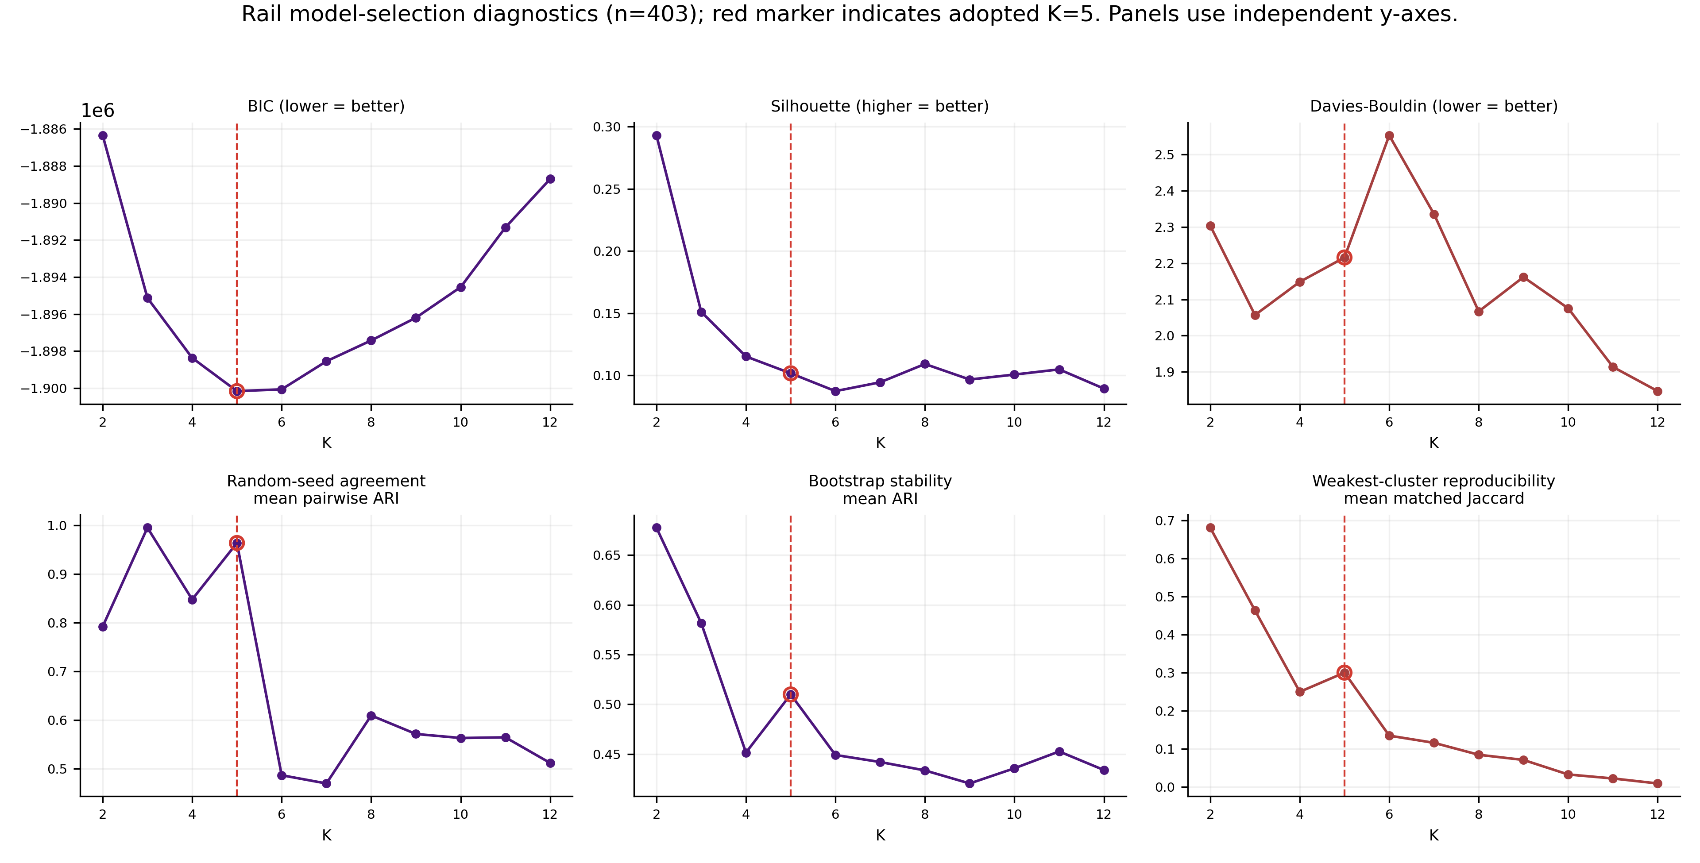
\includegraphics[width=\linewidth]{figures/v5_ch4_fig4.png}
\caption[Rail model-selection diagnostics]{Rail K selection evidence}
\end{figure}
\end{landscape}

\begin{landscape}
\begin{figure}[H]
\centering
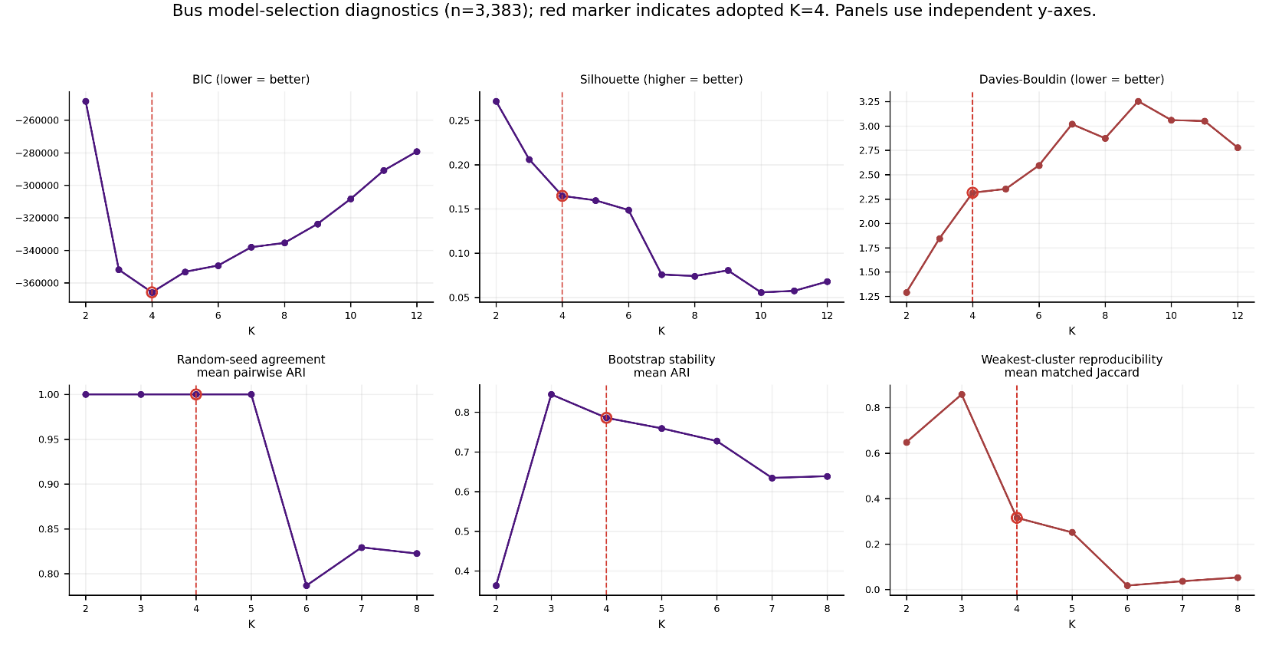
\includegraphics[width=\linewidth]{figures/v5_ch4_fig5.png}
\caption[Bus model-selection diagnostics]{Bus K selection evidence}
\end{figure}
\end{landscape}

Conditional on the fitted models, assignment ambiguity was low: 98.5\% of Rail stations and 99.0\% of Bus LSOAs had maximum posterior probabilities of at least 0.99. These probabilities describe assignment certainty within the fitted solution and should not be interpreted as evidence of resampling stability.

\section{Night-time Public Transport Usage Types}

Following the selection of the mode-specific cluster solutions, this chapter presents the identified night-time public transport usage types through their observed temporal profiles, post-clustering descriptors and spatial distributions. Rail and Bus were examined separately throughout because their analytical units and feature constructions differ.

\subsection{Five Night-time Usage Types: Rail System}

The following figures present the mean temporal profiles and spatial distribution of the five Rail clusters, respectively. The sections below summarise the main observed characteristics of each cluster.

\begin{figure}[H]
\centering
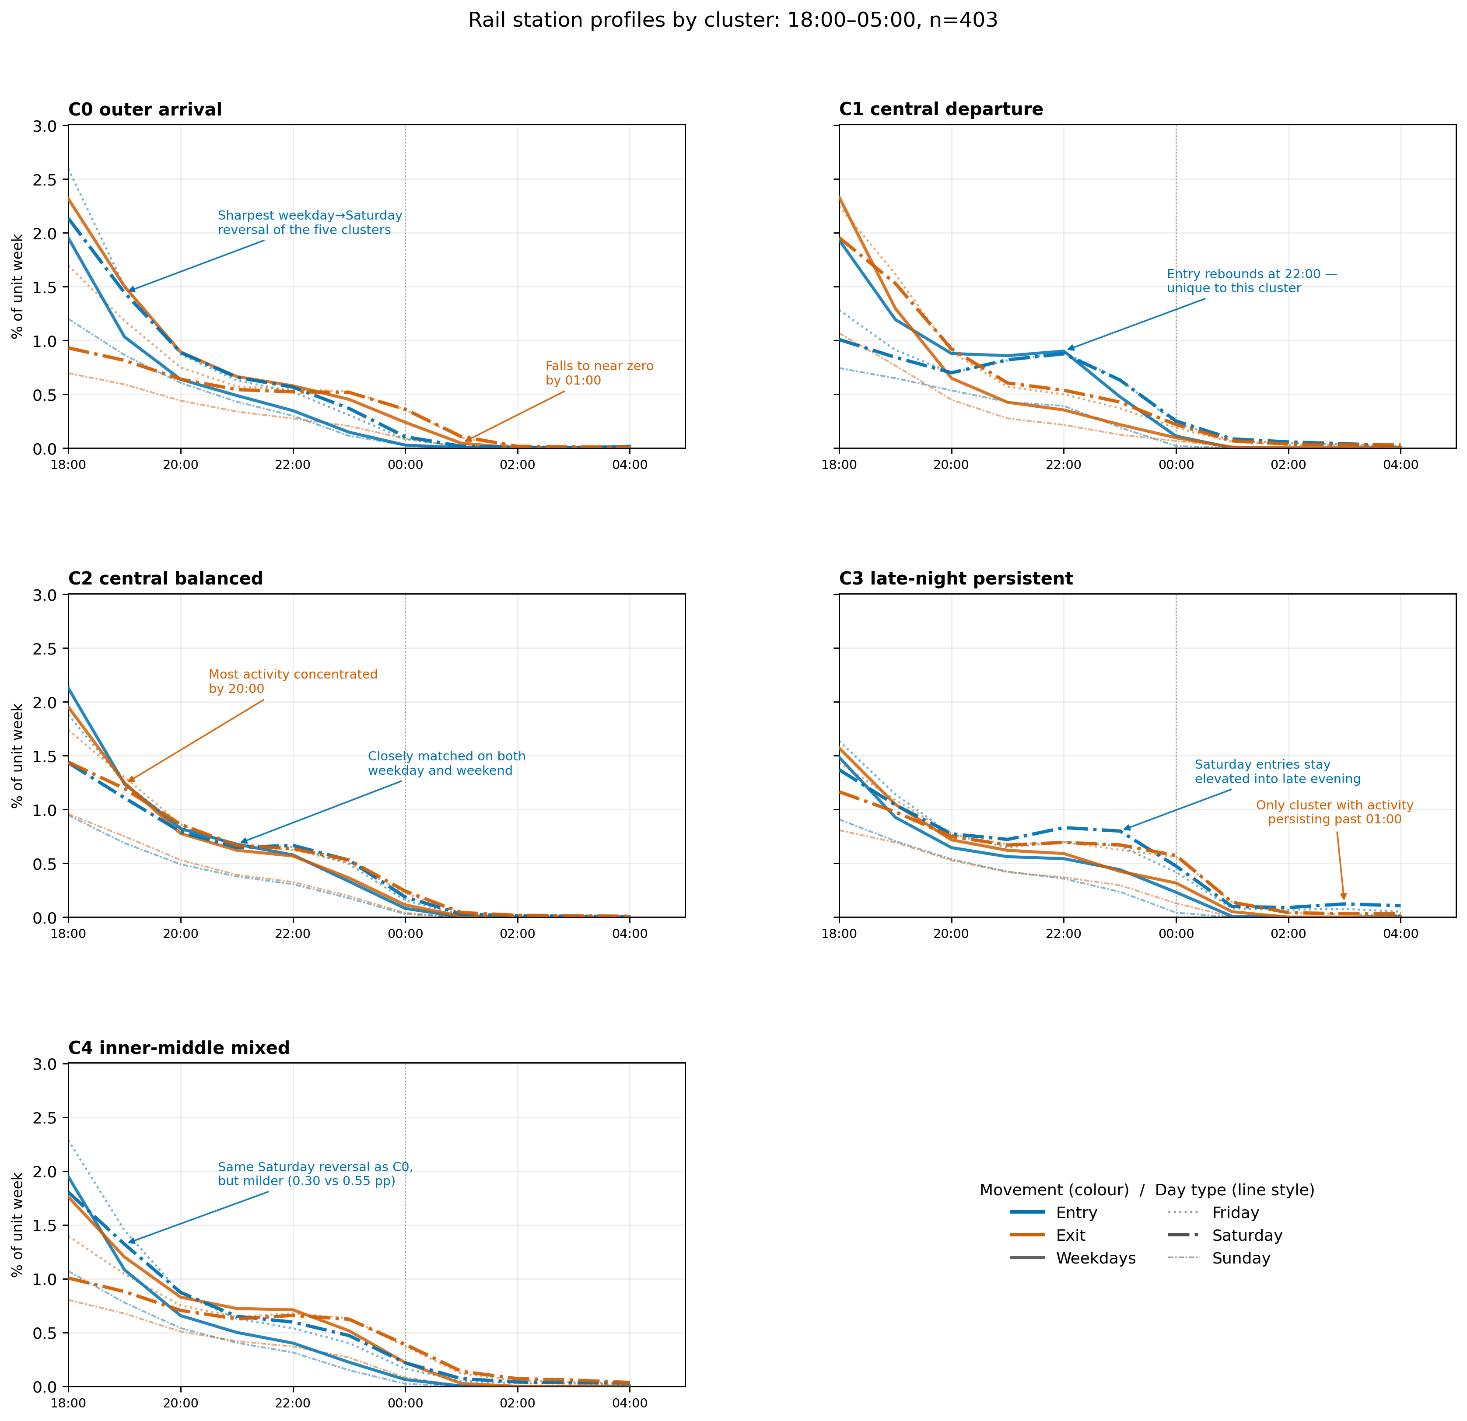
\includegraphics[width=\textwidth]{figures/v5_ch4_fig6.png}
\caption[Rail station temporal profiles]{Rail station temporal profiles (403 stations; K=5; 18:00--05:00). Colour distinguishes entries and exits; line style distinguishes day types; panels, labels and titles identify clusters.}
\end{figure}

\begin{figure}[H]
\centering
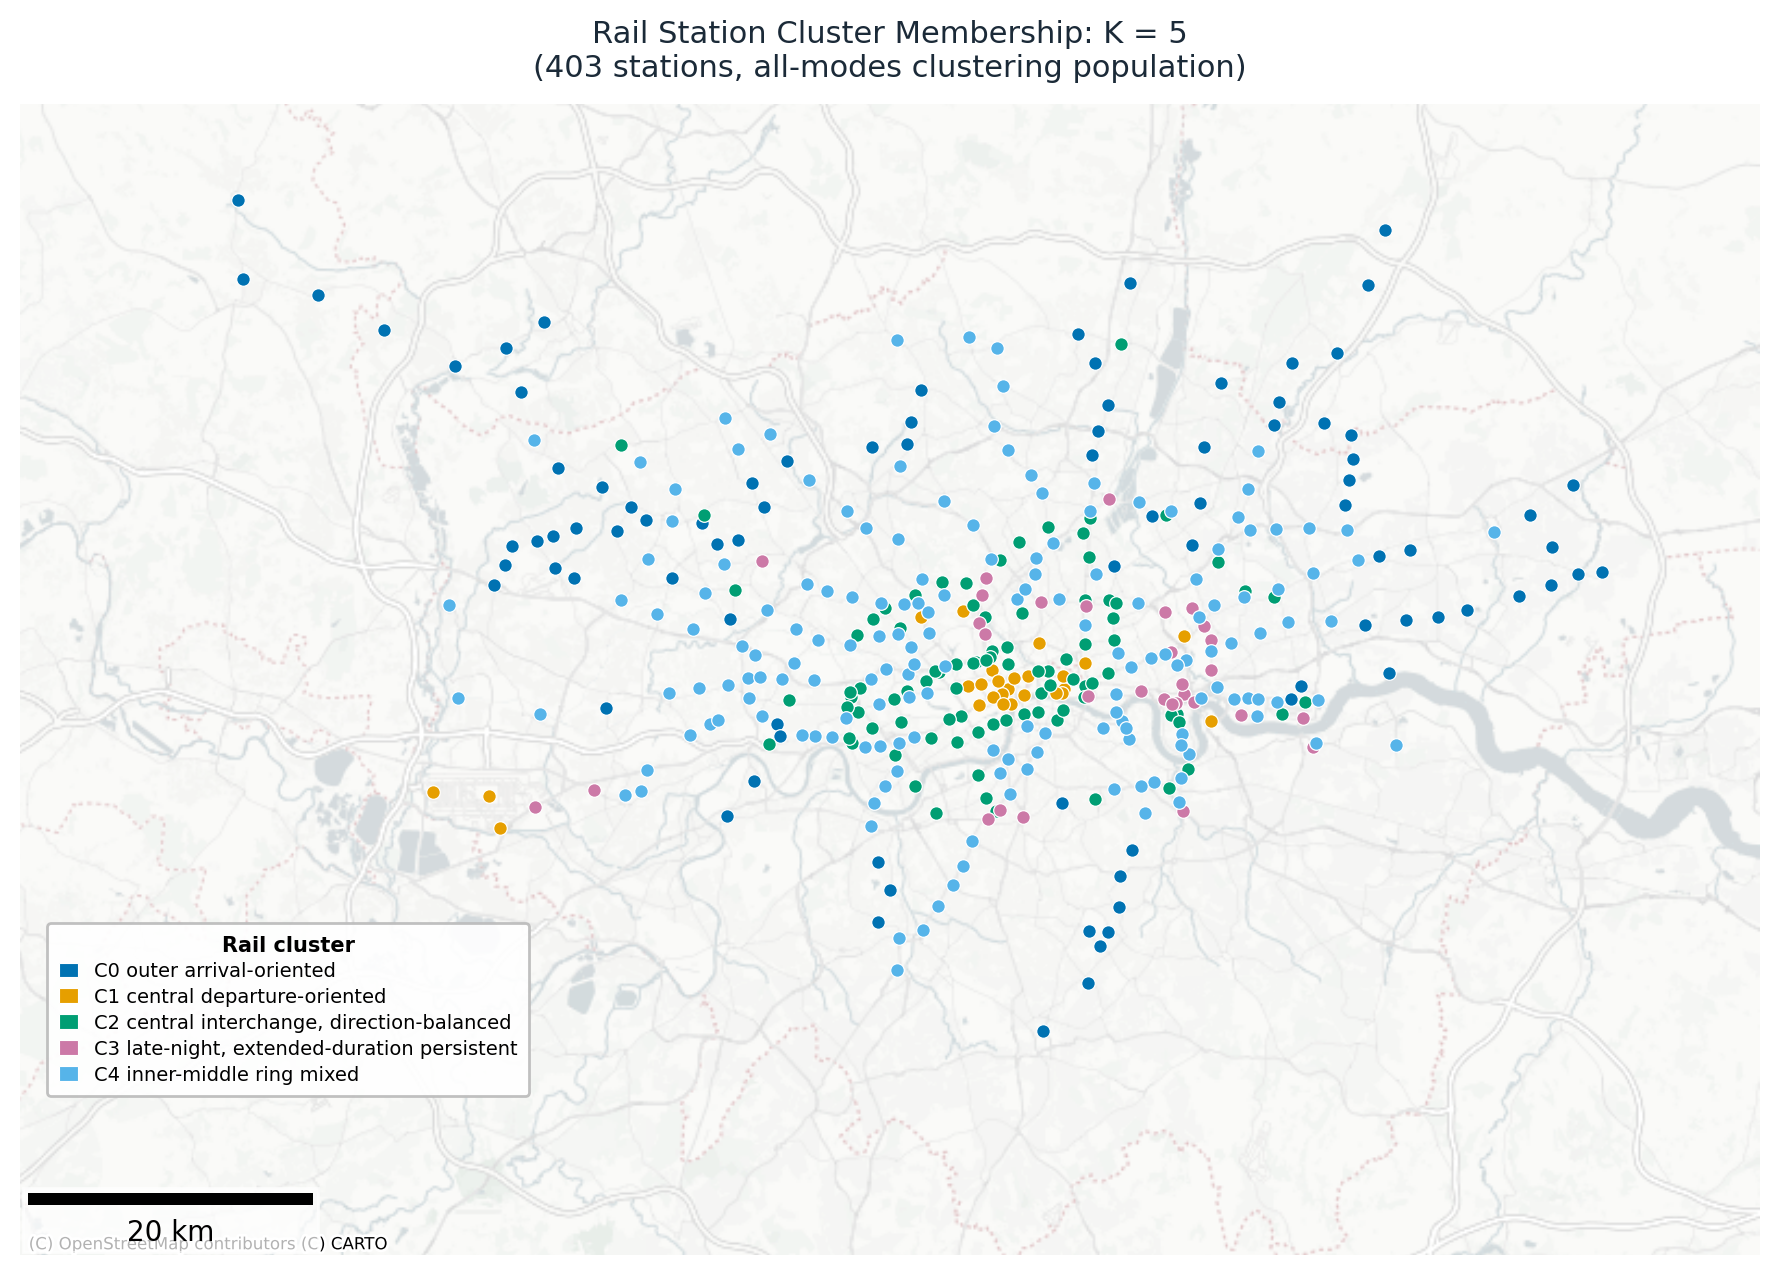
\includegraphics[width=\textwidth]{figures/v5_ch4_fig7.png}
\caption[Rail cluster map]{Rail cluster map: station-point analytical units}
\end{figure}

\begin{figure}[H]
\centering
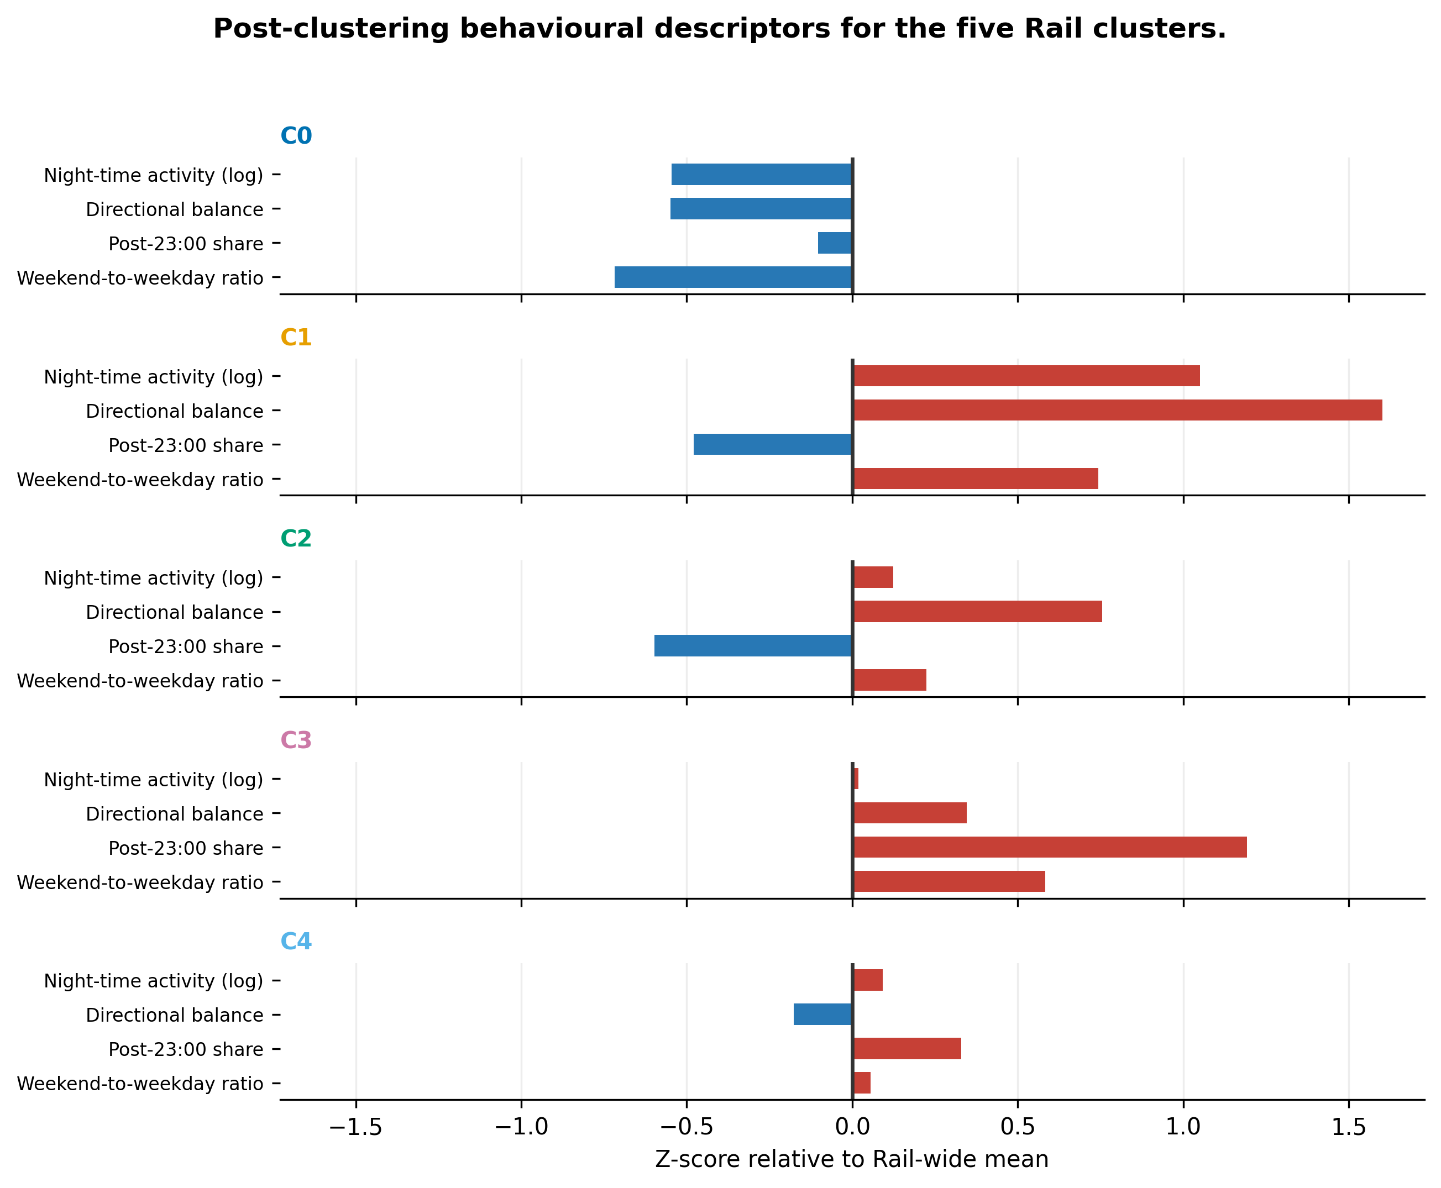
\includegraphics[width=\textwidth]{figures/v5_ch4_fig8.png}
\caption[Rail behavioural descriptors]{Post-clustering behavioural descriptors for the five Rail usage types. Values are cluster-mean z-scores relative to the Rail-wide mean and standard deviation. Positive and negative values indicate above- and below-average values, respectively; for directional balance, higher values indicate a stronger departure/entry orientation.}
\end{figure}

\textbf{C1: Night-time activity centres cluster (central departure) (n = 26).} C1 is tightly concentrated in central London, particularly around the West End and central activity areas. It includes major West End and central stations such as Oxford Circus and Piccadilly Circus, alongside a small number of more specialised transport nodes.

It records the highest overall night-time activity of all five clusters. The temporal profile shows strong exit activity between 18:00 and 20:00, followed by a distinctive rise in entries around 22:00. This later entry rebound is not visible to the same extent in the other clusters. The post-clustering descriptors also show the strongest positive directional balance, while the share of activity after 23:00 remains below the Rail average.

C1 is thus characterised by high-volume central activity and a pronounced departure orientation later in the evening, rather than by sustained deep-night use.

\textbf{C0: Outer arrival-oriented (n = 89).} C0 forms the clearest outer-London Rail type. Its stations are widely distributed along radial corridors at the edge of the network, with a mean distance of 17.76 km from central London.

Activity is concentrated in the early evening and declines rapidly thereafter, reaching very low levels by around 01:00. On weekdays, exits exceed entries, giving the cluster a clear arrival orientation. The balance changes most strongly on Saturday, when entries become relatively more prominent earlier in the evening and exits later at night.

Among the five clusters, C0 also has the lowest overall activity and the weakest relative weekend activity.

The combination of peripheral location, low activity and weekday exit dominance makes C0 the clearest outer arrival-oriented Rail type.

\textbf{C4: Inner--middle ring cluster (n = 167).} C4 is the largest Rail cluster and forms a broad band across inner and middle London. Its stations extend along several rail corridors and occupy an intermediate spatial position between the central clusters and the more peripheral C0.

The temporal profile shares some features with C0, including a mild shift in directional balance on Saturday, but the change is less pronounced. Activity also persists later into the night than in C0, reflected in an above-average post-23:00 share. Overall volume remains close to the Rail mean, while directional balance shows only a modest arrival tendency.

C4 is therefore better described as an inner--middle mixed type than as a strongly arrival-oriented cluster.

\textbf{C3: Late-night, extended-duration persistent (n = 31).} C3 is a small cluster located mainly across inner and eastern London. Unlike the larger Rail groups, its defining feature is not overall activity volume but the persistence of activity later into the night.

Its temporal profiles decline more slowly after the early evening, with Saturday entries remaining elevated into the late evening. C3 also shows the clearest continuation beyond 01:00 and has by far the highest post-23:00 activity share in the post-clustering descriptors.

This distinguishes C3 from both high-volume central clusters and larger arrival-oriented groups, which may reflect a combination of nearby night-time activities, interchange functions, local demand, and late-running services.

\textbf{C2: Central, direction-balanced cluster (n = 90).} C2 covers central London and a number of major inner-London interchange stations, including King's Cross St Pancras, Liverpool Street and London Bridge.

The entry and exit profiles remain closely aligned across most day types. Most activity is concentrated before 20:00 and declines steadily through the rest of the evening.

The close alignment of entry and exit activity distinguishes C2 from the stronger directional patterns of C1 and C0, making it a relatively high-activity central type without a pronounced arrival or departure bias.

\textbf{Overall Rail structure.} The Rail analysis identifies five relatively distinct night-time station types with different spatial location and temporal usage characteristics.

Across the five clusters, Rail usage differs in spatial position, directional balance, activity scale, the timing of evening activity and the extent to which activity continues later into the night. The clearest spatial contrast is between the high-activity central departure pattern of C1 and the low-activity outer arrival pattern of C0, while other clusters occupy less strongly directional or more temporally persistent positions.

C1 is the busiest and most centrally located type, yet its share of activity after 23:00 falls below the Rail average. C3, by contrast, records lower overall activity but the strongest late-night continuation and is concentrated mainly across inner and eastern London. The Rail typology therefore captures several forms of night-time station use that would not be distinguished by activity volume or spatial position alone.

\subsection{Four Night-time Area Profiles: Bus System}

Following figures show the mean temporal profiles and spatial distribution of the four Bus clusters. Although clustering was performed on CLR-transformed features, boarding and estimated-alighting shares are shown on original scale for interpretation.

Compared with Rail, the Bus profiles are less sharply differentiated. All four clusters show relatively high activity around 18:00, followed by a gradual evening decline, low activity after midnight, and some recovery in boarding around 04:00.

The main differences are in how quickly activity declines, how long it persists into the night, directional balance and overall activity level. More persistent patterns are concentrated mainly in central and inner London.

\begin{figure}[H]
\centering
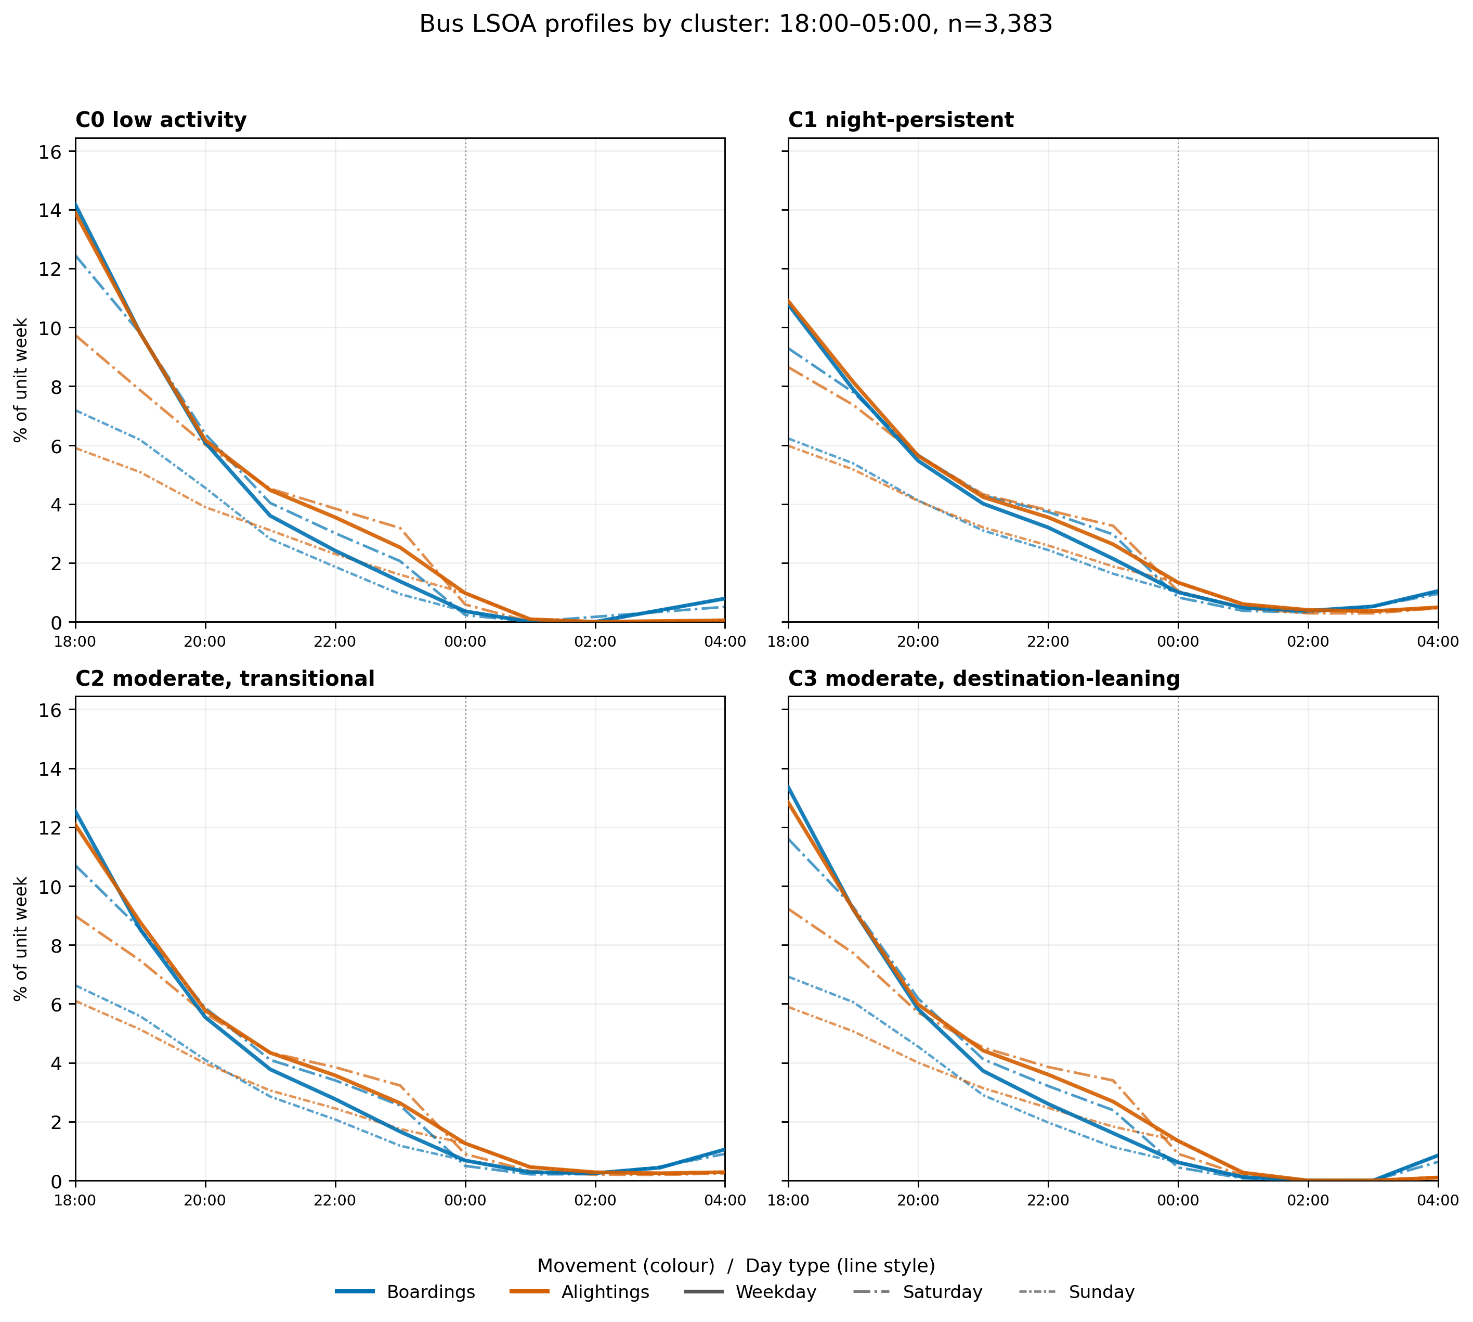
\includegraphics[width=\textwidth]{figures/v5_ch4_fig9.png}
\caption[Bus temporal profiles]{Bus temporal profiles (3,383 LSOAs; K=4; 18:00--05:00; threshold 33). Colour distinguishes boardings and estimated alightings; line style distinguishes day types.}
\end{figure}

\begin{figure}[H]
\centering
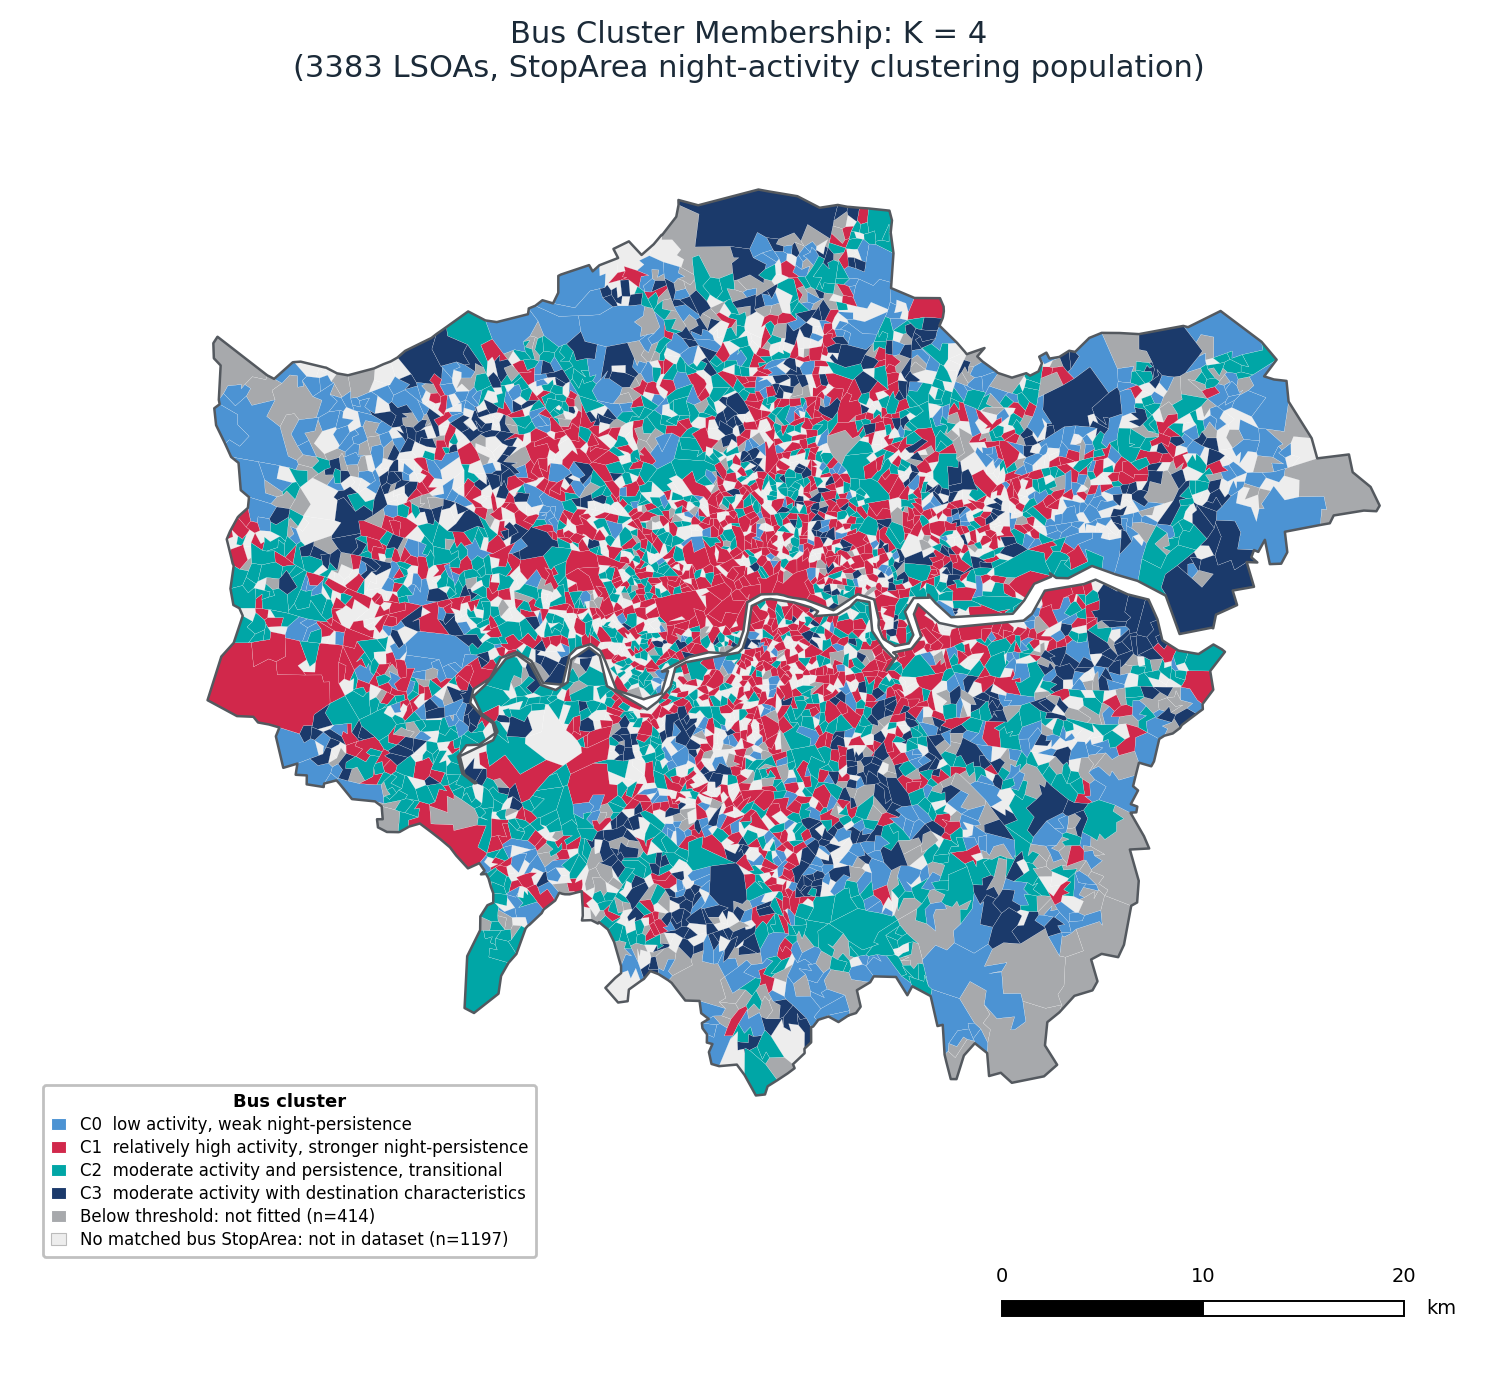
\includegraphics[width=\textwidth]{figures/v5_ch4_fig10.png}
\caption[Bus cluster map]{Bus cluster map: LSOA unit}
\end{figure}

\begin{figure}[H]
\centering
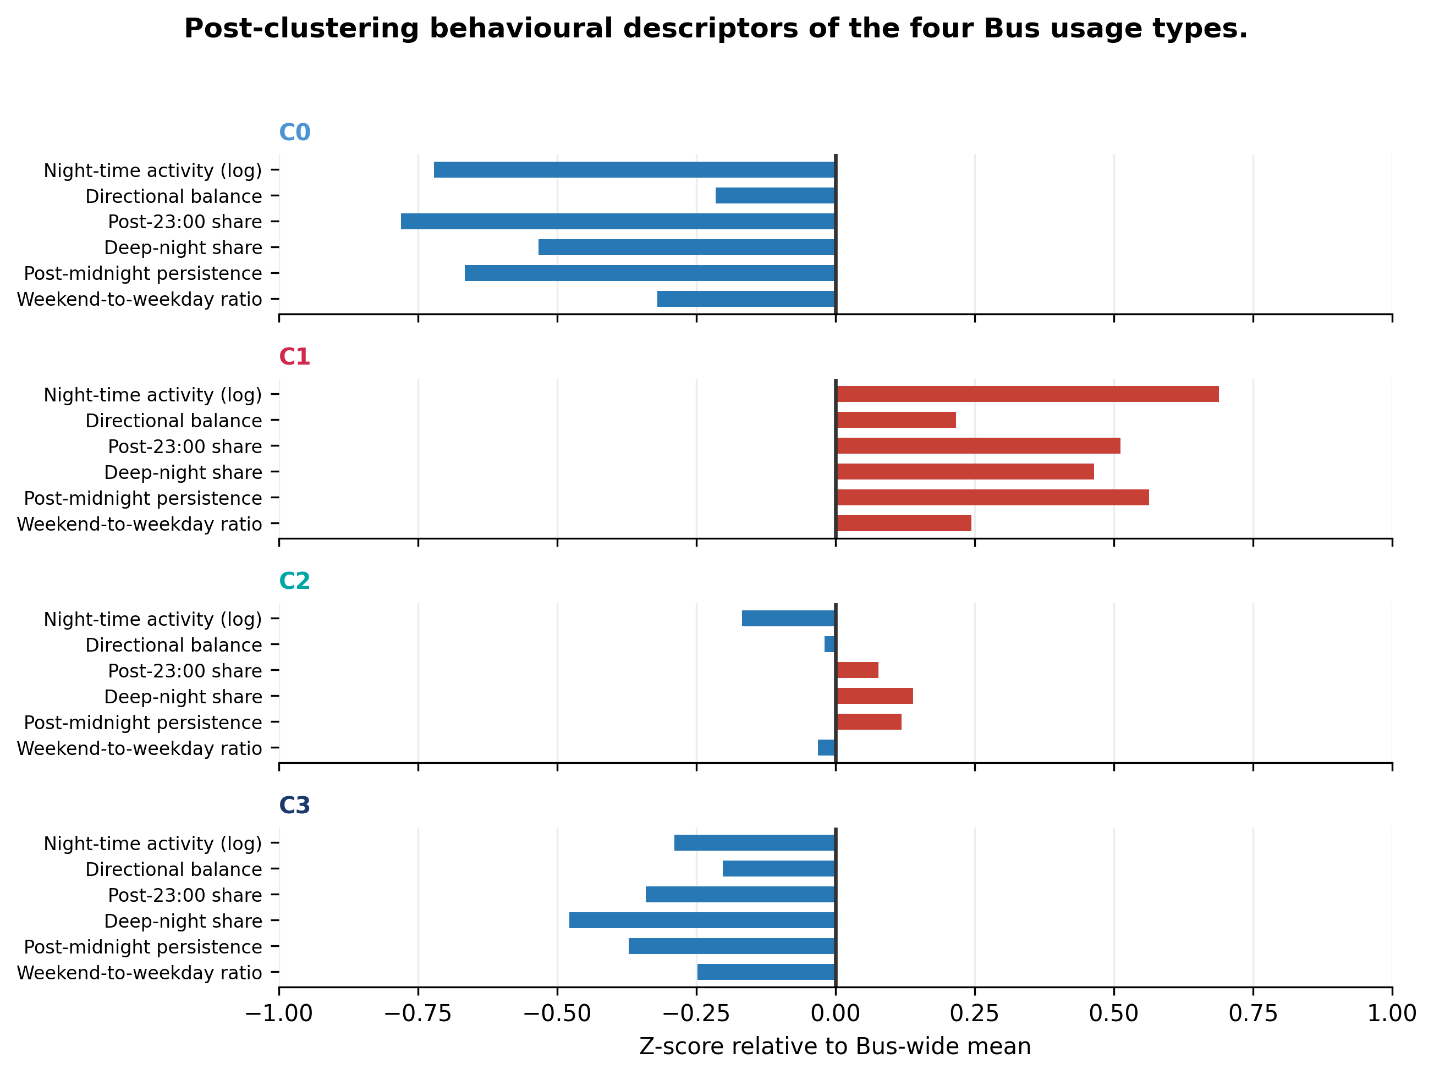
\includegraphics[width=\textwidth]{figures/v5_ch4_fig11.png}
\caption[Bus behavioural descriptors]{Standardised post-clustering behavioural descriptors of the four Bus usage types. Values show cluster-mean z-scores relative to the Bus-wide mean and standard deviation.}
\end{figure}

\textbf{C1: Relatively high activity, stronger night-persistence (n = 1,134).} C1 contains LSOAs with relatively high levels of night-time Bus activity and the strongest late-night persistence among the four clusters. Activity declines more gradually through the evening and remains comparatively sustained after midnight, with the highest post-midnight persistence value (0.155).

C1 is concentrated mainly in central and inner London, where these persistent patterns form the most continuous areas. The cluster also extends outward along several radial corridors, indicating that sustained late-night Bus activity is not confined to the central core.

\textbf{C2: Moderate activity and persistence, transitional (n = 1,069).} C2 is intermediate between the two endpoints: it retains more late-night activity than C0 but less than C1, and is distributed across inner, middle and some outer areas. Spatially C2 overlaps widely with the other clusters in space. This distribution supports its interpretation as a transitional profile between the two clearer endpoints rather than as a sharply localised area type.

\textbf{C3: Moderate activity with alighting-oriented estimated activity (n = 576).} C3 shows relatively stronger activity in the earlier part of the night, followed by a clearer decline after 23:00. Within the overlapping middle of the Bus gradient, it differs from C2 through a more alighting-oriented balance of estimated activity. Spatially, C3 occurs more often outside the central core and extends across several outer-London LSOAs.

\textbf{C0: Low activity, weak night persistence (n = 604).} C0 defines the low-activity endpoint. Its profile falls most rapidly from the early evening and records the lowest persistence after midnight (0.031), making it the clearest early-declining bus type.

It is concentrated mainly in outer suburban London, in contrast to the more central and persistent C1 pattern.

\textbf{Overall Bus structure.} The four Bus clusters are differentiated mainly by how long activity persists into the night rather than in entirely different temporal shapes. C1 and C0 mark the clearest endpoints. C1 retains the highest level of activity after midnight (0.155), while C0 declines earliest and has the lowest persistence (0.031); C2 occupies an intermediate position. This variation broadly follows a centre-to-outer London gradient.

C3 adds a second distinction: it is similar to C2 in overall activity level, but shows a more alighting-oriented balance of estimated activity. The difference between them is one of direction rather than persistence. But because Bus alighting is estimated rather than observed, this distinction is interpreted more cautiously than the persistence gradient.

\section{Relationship with Area Context}

The clustering results have shown the night-time usage types, spatial distribution, and cross-system differences for the Rail and Bus systems. The following analysis relates these usage characteristics to LNWC and the wider city background variables, and considers what these associations suggest.

\subsection{Correspondence with the Geography of Night Work}

Figures 4.9 and 4.10 compare each transport type with its own eligible LNWC benchmark (ER=1). Night-work geography is associated with both typologies.

Rail's node rhythms correspond to several distinct night-work settings, while Bus variation aligns with a broader contextual gradient.

\subsubsection{Rail Clusters and LNWC}

\begin{figure}[H]
\centering
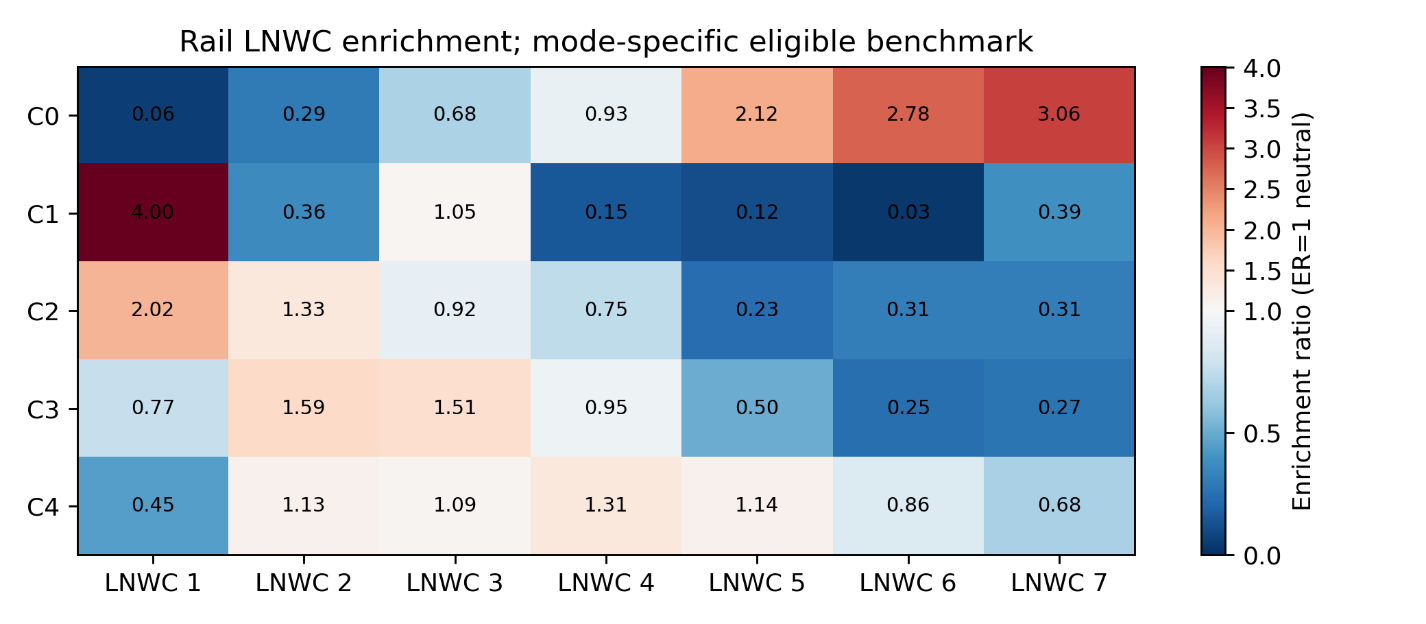
\includegraphics[width=\textwidth]{figures/v5_ch4_fig12.png}
\caption[Rail LNWC enrichment]{Rail LNWC enrichment ratios, using 800\,m equal-station catchment context and the 389-station eligible-Rail benchmark (ER=1 neutral).}
\end{figure}

The seven-part LNWC compositions differed systematically across the five Rail clusters. The observed between-cluster compositional differentiation was greater than expected under random reassignment of the fixed cluster labels ($R^2 = 0.263$, permutation $p = .001$, $n = 389$; 999 permutations). This omnibus result indicates an association between the Rail typology and LNWC composition, while the enrichment ratios below show which LNWC types contributed to the observed differences.

The strongest Rail enrichment links C1 to LNWC 1, Thriving night-worker central hubs (ER = 3.98). The temporal profile establishes that C1 is busy and departure-oriented; the LNWC association places that pattern in the most intensive central night-work setting in London.

C0 sits at the opposite end of the LNWC distribution, with its strongest enrichment in LNWC 7, Night-work periphery (ER = 3.06), alongside LNWC 5 and LNWC 6. These areas all fall within the category of those identified by LNWC as having relatively low levels of night-time activity. This result is consistent with a relatively weak night-time activity context and arrival-oriented profile around these stations.

C4 has a comparatively mixed LNWC profile, consistent with its broad inner-middle-ring spatial distribution rather than one dominant night-work setting.

C3 is most enriched in LNWC 2, Inner suburbs, high night business (ER = 1.59), and LNWC 3, Inner suburbs, low night business (ER = 1.51), with no comparable concentration in LNWC 1. This is notable because C3 was identified earlier as the Rail cluster with the strongest late-night persistence and the highest post-23:00 activity share. This mismatch warrants further examination in the following section.

C2 is also enriched in central and inner-London night-work contexts, including LNWC 1 and LNWC 2, but its contextual profile is more mixed than C1's.

Taken together, LNWC correspondence is strongest at the two ends of the Rail typology. C1 and C0 both exceed an enrichment ratio of 3.0 for their dominant LNWC types, while the association weakens for C2 (2.01), C3 (1.59) and especially C4, which has no dominant type. As these three intermediate clusters contain the majority of analysed stations, LNWC distinguishes only part of the wider Rail typology.

This pattern is consistent with the overall $R^2$ of 0.263: night-work context is associated with Rail usage type, but does not account for its full variation. The next section examines whether broader urban background characteristics help distinguish the less clearly separated clusters.

\subsubsection{Bus Clusters and LNWC}

\begin{figure}[H]
\centering
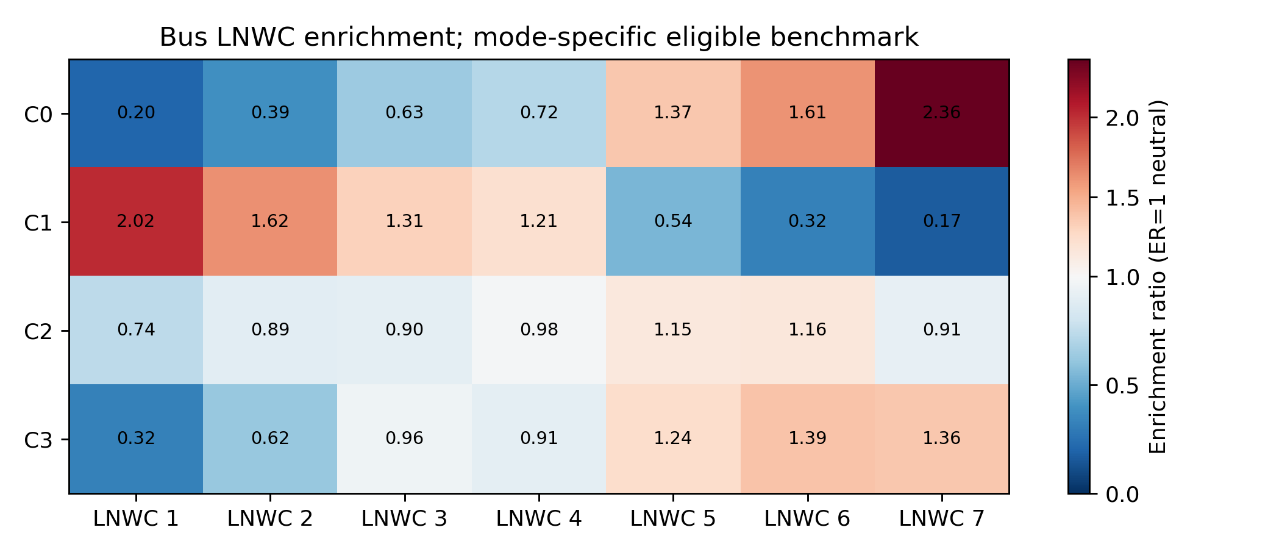
\includegraphics[width=\textwidth]{figures/v5_ch4_fig13.png}
\caption[Bus LNWC enrichment]{Bus LNWC enrichment ratios (ER=1 neutral).}
\end{figure}

A Pearson chi-square test indicated an association between the four Bus clusters and the seven LNWC types, $\chi^2 (18, n = 3{,}383) = 647.50$, $p < .001$, Cramér's V = 0.253, indicating that the association was present but not sufficient to treat Bus cluster membership and LNWC type as equivalent classifications.

C1 and C0 form near mirror images across the LNWC sequence: C1 declines from 2.02 to 0.17 from centre to periphery, while C0 rises from 0.20 to 2.36. C3 shows a weaker peripheral tendency than C0, whereas C2 remains close to neutral throughout (0.74--1.16).

The association again concentrates at the ends of the typology rather than in its middle. In particular, it does little to distinguish C3 from C2 along the directional dimension that separates them in the transport data.

\subsection{Relation to City Background Variables}

The following analysis characterises the context surrounding each cluster. The omnibus tests showed that the contextual distributions differed across clusters for all 20 Bus indicators and for 19 of the 20 Rail indicators after mode-specific Benjamini--Hochberg correction. The exception was the Rail Asian population share (BH-adjusted $p = .054$).

The strongest Rail differentiation concerned car access, younger-adult composition, households with dependent children, private renting and POI intensity.

For Bus, the strongest differences concerned car access, younger-adult composition, POI intensity, private renting and accommodation-and-food employment.

The cluster-versus-rest tests further identified where these overall differences occurred. After Benjamini--Hochberg correction, 63 of the 100 Rail contrasts and 66 of the 80 Bus contrasts remained statistically significant. The z-score panels show the direction of cluster-mean deviation, while rank-biserial correlations quantify the corresponding cluster-versus-rest contrasts. Full omnibus results are reported in Appendix Table~\ref{tab:appA3}, with Rail and Bus cluster-versus-rest effect sizes in Tables~\ref{tab:appA4} and \ref{tab:appA5}, respectively.

\begin{table}[H]
\centering
\small
\resizebox{\textwidth}{!}{%
\begin{tabular}{@{}l p{5cm} r r l@{}}
\toprule
Mode & Contextual variable & Kruskal--Wallis $H$ & $\varepsilon^2$ & BH-adjusted $p$ \\
\midrule
Rail & No-car household share & 165.10 & .420 & $<$.001 \\
Rail & Age 20--34 share & 144.35 & .365 & $<$.001 \\
Rail & Dependent-children share & 131.39 & .332 & $<$.001 \\
Rail & Private-rented share & 105.12 & .263 & $<$.001 \\
Rail & Log POI count & 102.75 & .257 & $<$.001 \\
Bus & No-car household share & 735.42 & .217 & $<$.001 \\
Bus & Age 20--34 share & 583.94 & .172 & $<$.001 \\
Bus & Log POI count & 518.16 & .152 & $<$.001 \\
Bus & Private-rented share & 494.95 & .146 & $<$.001 \\
Bus & Accommodation-and-food employment share & 353.97 & .104 & $<$.001 \\
\bottomrule
\end{tabular}%
}
\caption[Strongest contextual differences]{Strongest contextual differences (top five) across the fixed Rail and Bus clusters.}
\end{table}

\subsubsection{Rail Area Context}

Figure 4.14 provides two complementary views of regional background context. The effect-size ranking identifies the dimensions that most clearly differentiate the fixed clusters within each mode; the z-score displays show the direction of each cluster's profile relative to its mode-wide mean.

\begin{figure}[H]
\centering
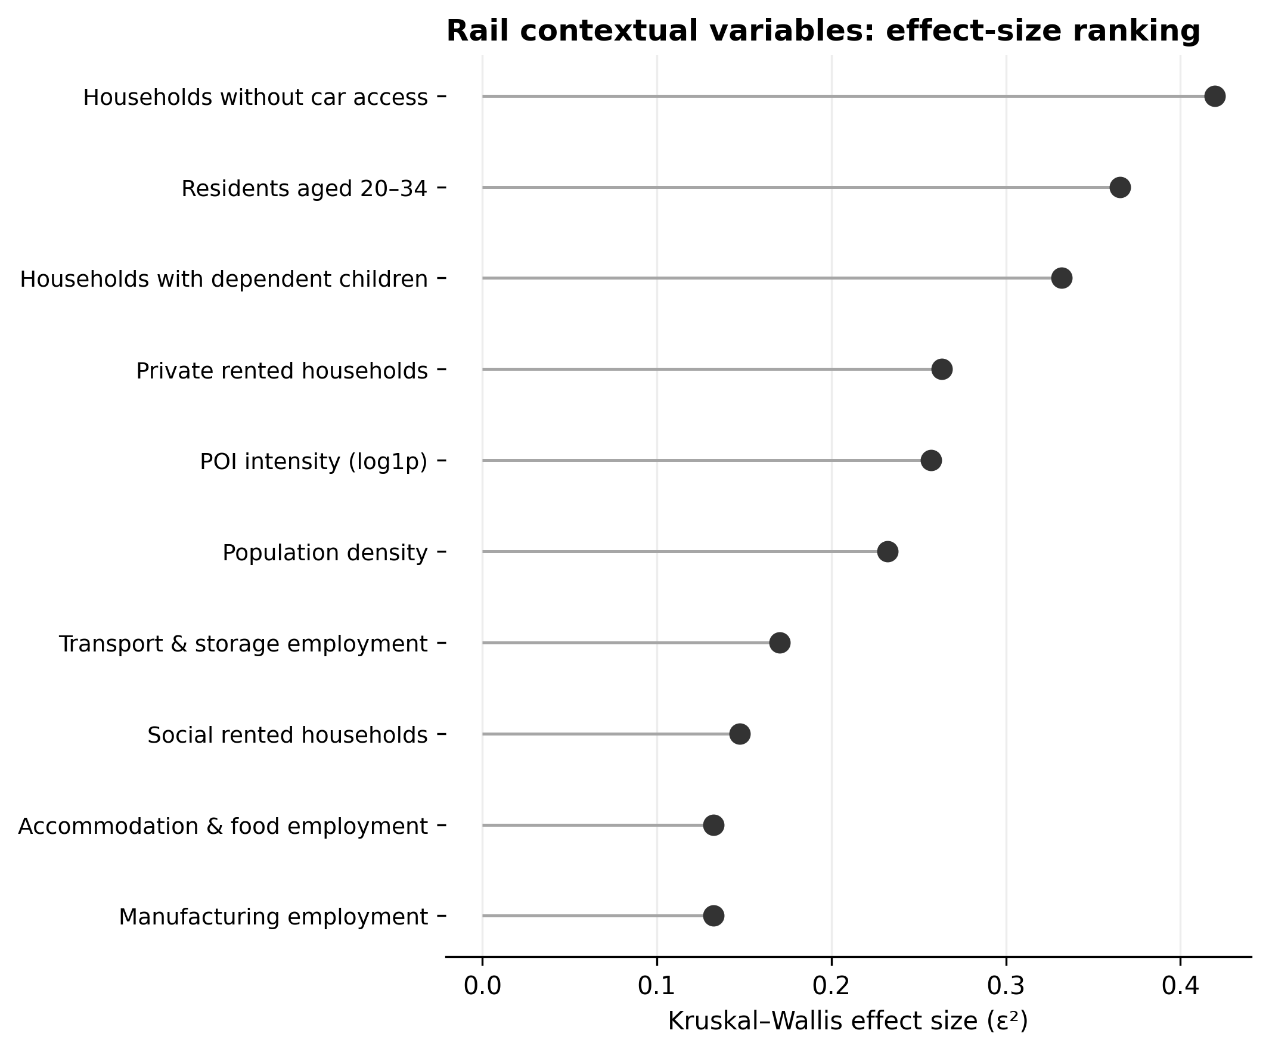
\includegraphics[width=0.95\textwidth]{figures/v5_ch4_fig14.png}
\caption[Rail contextual effect-size ranking]{Contextual indicators with the largest Kruskal--Wallis effect sizes across the five Rail usage types. Effect sizes are measured using $\varepsilon^2$; larger values indicate stronger between-cluster differentiation.}
\end{figure}

\clearpage
\begin{landscape}
\begin{figure}[H]
\centering
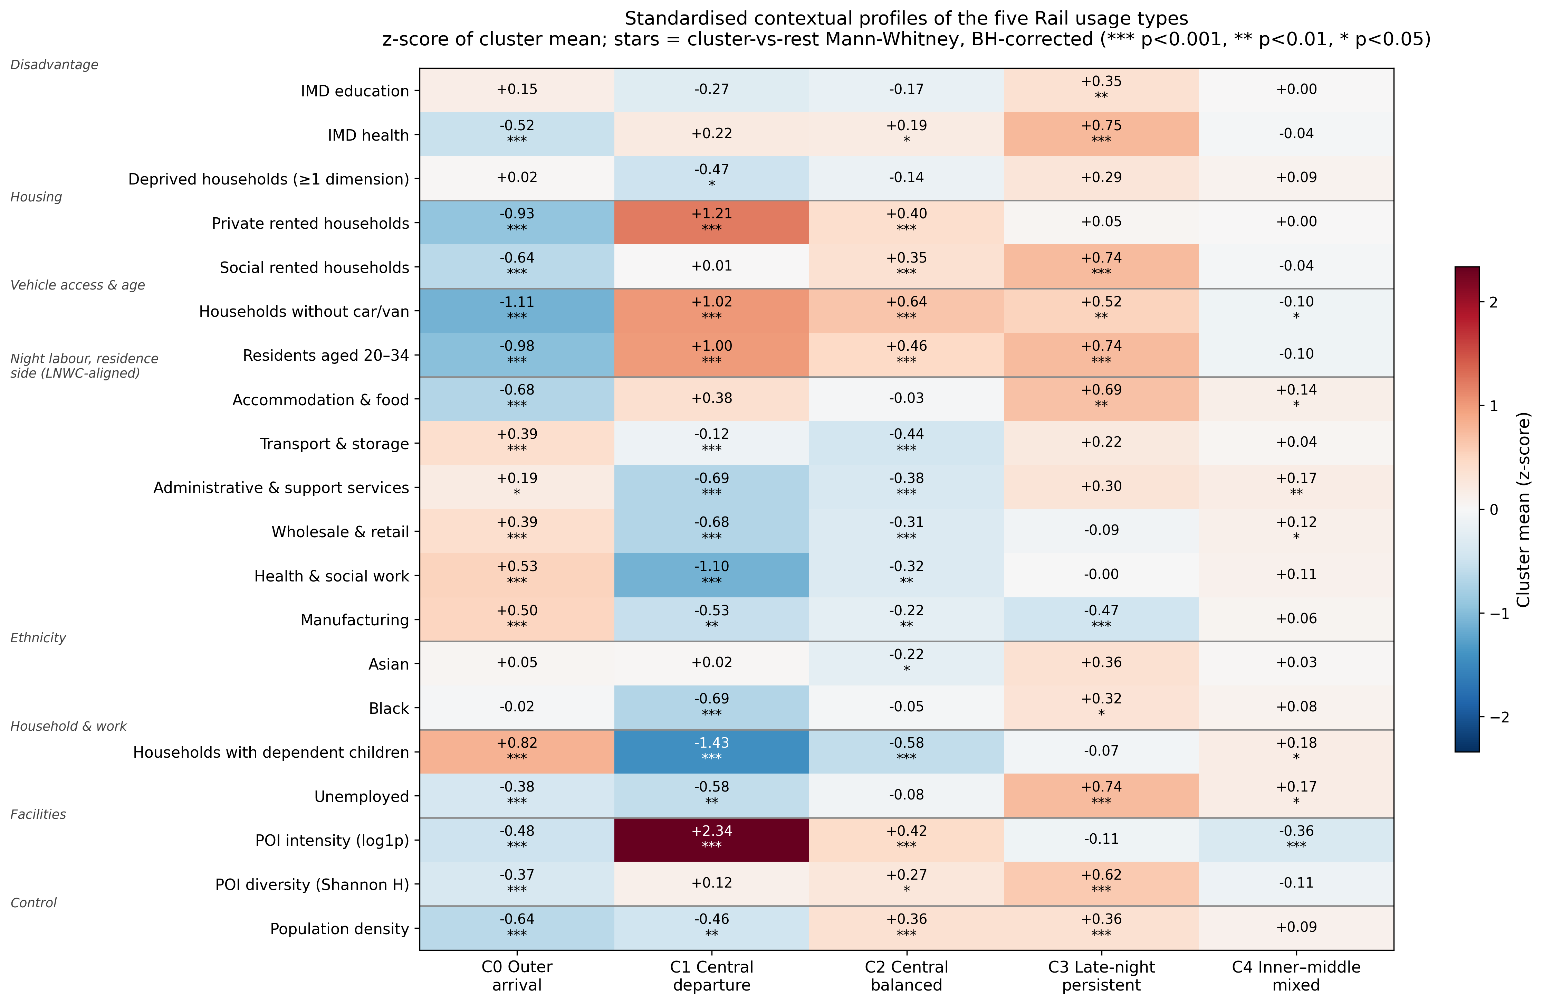
\includegraphics[width=\linewidth,height=0.76\textwidth,keepaspectratio]{figures/v5_ch4_fig15.png}
\caption[Rail contextual profiles]{Standardised contextual profiles of the five Rail usage types. Cell values show cluster-mean z-scores for each contextual indicator relative to all eligible Rail stations. Positive values indicate above-average and negative values below-average contextual characteristics within Rail. Dots indicate significant cluster-versus-rest Mann--Whitney tests after Benjamini--Hochberg correction. The colour scale is mode-specific.}
\end{figure}
\end{landscape}

For Rail, vehicle access, age, household composition, tenure and POI intensity provide the strongest overall contextual differentiation. The cluster-level profiles reveal that these dimensions combine into multiple socio-spatial patterns.

Night-time activity centres (C1) are located in younger, more privately rented and amenity-intensive surroundings, with particularly high POI intensity. They also have a higher prevalence of households without cars and fewer households with dependent children, providing a clearer picture of the urban context surrounding C1 stations.

Outer arrival-oriented stations (C0) are associated with a more suburban household profile, including more households with dependent children, fewer car-free households and a smaller share of younger adults. The catchments also have relatively high resident employment in transport and storage, wholesale and retail, health and social work, and manufacturing. This contrasts with the LNWC pattern: C0 lies mainly in peripheral areas with relatively low recorded night-time activity, yet its surrounding residential areas contain comparatively high employment in several industries associated with night-time work.

The inner--middle ring cluster (C4) remains close to the Rail-wide mean across most variables, consistent with its broad spatial coverage.

The central, direction-balanced cluster (C2) retains a more moderate central profile, sharing C1's centrality without its intensity.

Late-persistent stations (C3) return to the mismatch noted earlier. The catchments show higher levels of health deprivation, social renting and unemployment, alongside a larger share of younger adults and residents employed in accommodation and food services.

These characteristics distinguish C3 from both the amenity-intensive central profile of C1 and the more family-oriented outer profile of C0. C3 thus provides a distinctive case for considering how sustained late-night transport use relates to socio-spatial conditions beyond the concentration of night-time work alone.

No-car prevalence requires more cautious interpretation. It is highest around central C1 stations, but these catchments are often highly commercial and contain relatively small residential populations, making resident-based measures less representative of the wider station environment. For this reason, the observed pattern is better interpreted as a characteristic of the central-area context rather than as a direct indication of passenger characteristics.

\subsubsection{Bus Area Context}

\begin{figure}[H]
\centering
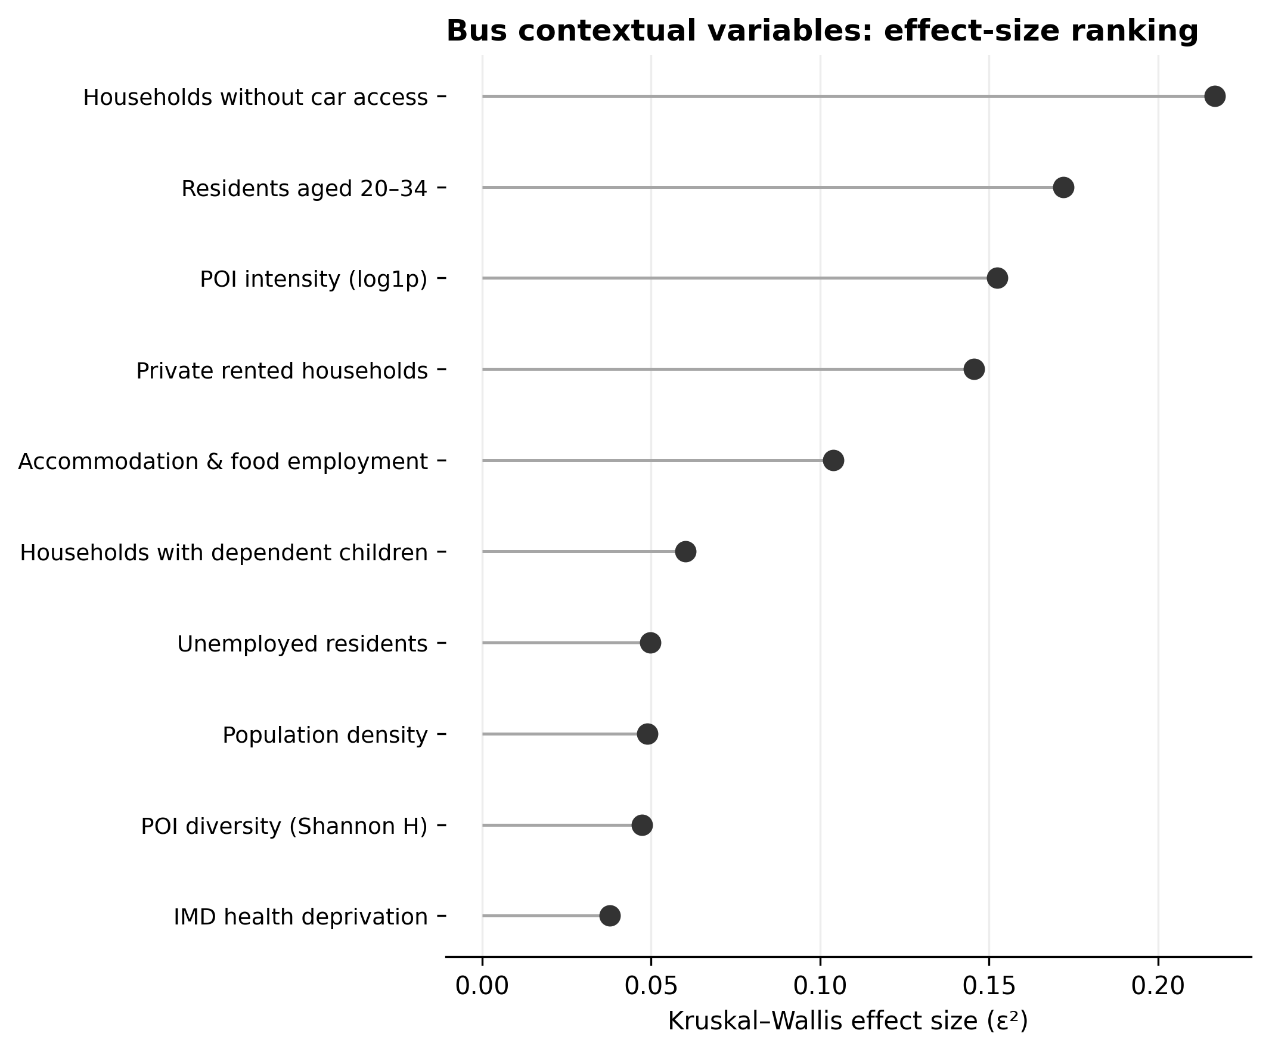
\includegraphics[width=0.95\textwidth]{figures/v5_ch4_fig16.png}
\caption[Bus contextual effect-size ranking]{Contextual indicators with the largest effect sizes across Bus usage types.}
\end{figure}

\clearpage
\begin{landscape}
\begin{figure}[H]
\centering
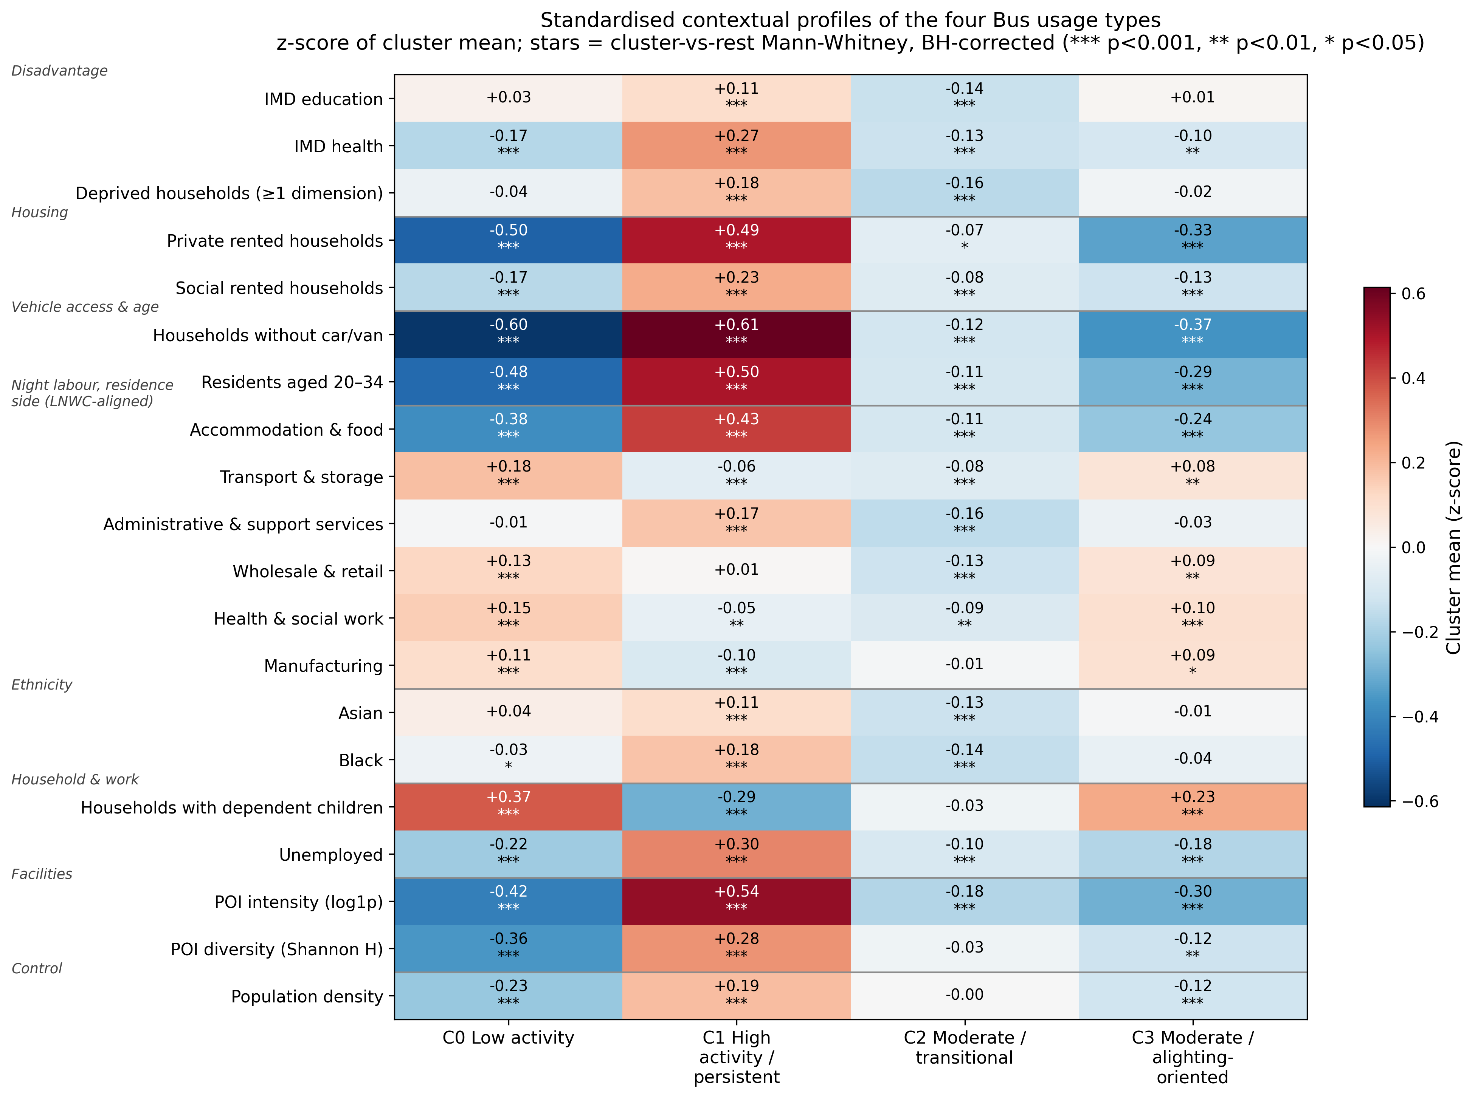
\includegraphics[width=\linewidth,height=0.76\textwidth,keepaspectratio]{figures/v5_ch4_fig17.png}
\caption[Bus contextual profiles]{Standardised contextual profiles of the four Bus usage types. Cell values show cluster-mean z-scores for each contextual indicator relative to all eligible Bus-served LSOAs. Positive values indicate above-average and negative values below-average contextual characteristics within Bus. Dots indicate significant cluster-versus-rest Mann--Whitney tests after Benjamini--Hochberg correction. The colour scale is mode-specific.}
\end{figure}
\end{landscape}

For Bus, car access, younger-adult composition, POI intensity and private renting provide contextual distinctions across the area activity-persistence gradient.

The persistent central/inner C1 cluster is associated with younger populations, more private renting, higher no-car prevalence and greater POI intensity, alongside somewhat higher deprivation-related indicators.

The early-declining outer C0 cluster shows the opposite pattern and a higher share of households with dependent children.

Despite its lower activity and earlier decline, C0 shows above-average residence-based employment in several sectors associated with night-time work, including transport and storage, wholesale and retail, health and social work, and manufacturing, while accommodation and food employment is lower.

C2 and C3 remain intermediate across most of the 20-variable profile, matching their overlapping temporal and spatial positions.

\section{Summary of Results}

The analysis revealed different forms of night-time organisation across the two modes. Rail comprised relatively differentiated types distinguished by direction, spatial position, activity scale and late-night continuation, whereas Bus followed a smoother activity--persistence gradient from central and inner London towards earlier-declining outer areas.

These mode-specific rhythms were also embedded in contrasting socio-spatial contexts. Rail types were associated with distinct combinations of night-work, household, housing, employment and facility characteristics, while Bus context varied more gradually along a centre-to-periphery gradient. These findings provide the basis for the interpretation developed in Chapter 5.
